\begin{myframe}{Matrix DFT}
\centering
\begin{align*}
\fn(k)&=\dft = (\wn{0k},\dots,\wn{(N-1)k}) \xv^T \\
\wvm &= \begin{bmatrix}
    \wn{0\times0}       & \wn{0\times1} & \dots & \wn{0\times(N-1)} \\
    \wn{1\times0}       & \wn{1\times1} &\dots & \wn{1\times(N-1)} \\
    \hdotsfor{4} \\
    \wn{(N-1)\times0}   & \wn{(N-1)\times1} &  \dots & \wn{(N-1)\times(N-1)}
\end{bmatrix}\\
(\wvm_{(k,n)} &=\wn{k \times n})\\
\fn(k) &= (\wvm \xv^T)_k 
\end{align*}
\begin{block}{}
\begin{equation*}
\fnv \xv = \wvm \xv^T 
\end{equation*}
\end{block}

\end{myframe}

\begin{myframe}{FFT Review}
\centering

\begin{block}{Calculating $\fn(k)$ for all $k$}
\begin{enumerate}
\item Split $x(n)$ into $x_{odd}(n)$ and $x_{even}(n)$.
\item Calculate $\fnneven(k)$ and $\fnnodd(k)$ for all $k$
\item Calculate $\fn(k)$ for all $k$ as:
\begin{equation}
\fn (k) = \begin{cases}
\fnneven (k) + \wn{k} \fnnodd (k) & \mbox{if } k=0,\dots,N/2-1 \\
\fnneven (k') - \wn{k'} \fnnodd (k') & \mbox{if } k=N/2,\dots,N-1 
\end{cases}
\end{equation}
($k=k'+N/2$)
\end{enumerate}
\end{block}

\begin{block}{Factorization}
Operations \textbf{1}, \textbf{2} and \textbf{3} can be expressed as a matrix too.
\end{block}

\end{myframe}


\begin{myframe}{Matrix FFT: Factorization}
\centering

\begin{align*}
\fnv \xv &=  
\begin{bmatrix}
\ve{I} &  \ve{D_N} \\
\ve{I} &  \ve{-D_N}
\end{bmatrix}  
\begin{bmatrix}
\fnnv & 0 \\
0 & \fnnv 
\end{bmatrix}  
\begin{bmatrix}
1 & 0 & 0 & 0 & \dots  \\
0 & 0 & 1 & 0 & \dots \\
\vdots & \vdots & \vdots &  \vdots &  \\
0 & 1 & 0 & 0 &  \dots  \\
0 & 0 & 0 & 1 & \dots \\
\vdots & \vdots & \vdots & \vdots & 
\end{bmatrix}  \xv
\\
&=  
\cmv_N
\begin{bmatrix}
\fnnv & 0 \\
0 & \fnnv
\end{bmatrix}  
\pmv_N
\xv
\end{align*}

\begin{block}{D diagonal, with twiddle factors}
\begin{equation}
\ve{D_{N(i,i)}}= \wn{i}, \qquad i=0,\dots, N-1
\end{equation}
\end{block}

\end{myframe}

\begin{myframe}{Matrix FFT: Factorization}
\centering

\begin{align*}
\fnv \xv &=  
\cmv_N
\cmv_{N/2}
\begin{bmatrix}
\fnnnv & 0 & 0 & 0\\
0 & \fnnnv & 0 & 0 \\
0 & 0 & \fnnnv & 0  \\
0 & 0 & 0 & \fnnnv\\
\end{bmatrix}  
\pmv_{N/2}
\pmv_N \xv\\
&=
\cmv_N
\cmv_{N/2}
\cmv_{N/2^2}
\dots
\cmv_{1}
\ve{I}
\pmv_{1}
\dots
\pmv_{N/2^2}
\pmv_{N/2}
\pmv_N \xv\\
&= 
\cmv_N
\cmv_{N/2}
\cmv_{N/2^2}
\dots
\cmv_{1}
\pmv_{1}
\dots
\pmv_{N/2^2}
\pmv_{N/2}
\pmv_N \xv\\
\end{align*}

\end{myframe}
\begin{myframe}{Matrix FFT: Iterative}
\centering

\begin{block}{Calculating $\fn(k)$}
\begin{enumerate}
\item Apply $\log_2(n)$ permutations $\pmi$ to $\xv$ to obtain $\xv'$
\item Apply $\log_2(n)$ combination operations $\cmi$ to $\xv'$ to obtain $\fn(\xv)$
\end{enumerate}
\end{block}


\begin{block}{Running time}
\begin{itemize}
\item Even though each permutation and combination operation is represented by an N-by-N matrix, it can be applied in $O(n)$ time
\item Each item above is therefore $O(n \log(n))$
\item Total running time is still $O(n \log(n))$
\end{itemize}
\end{block}

\end{myframe}

\begin{myframe}{Iterative FFT: Implementation}
\centering
\lstinputlisting[basicstyle=\small\ttfamily]{code/facuft_iterative.m}
\end{myframe}

\begin{myframe}{Iterative FFT: Output}
\centering
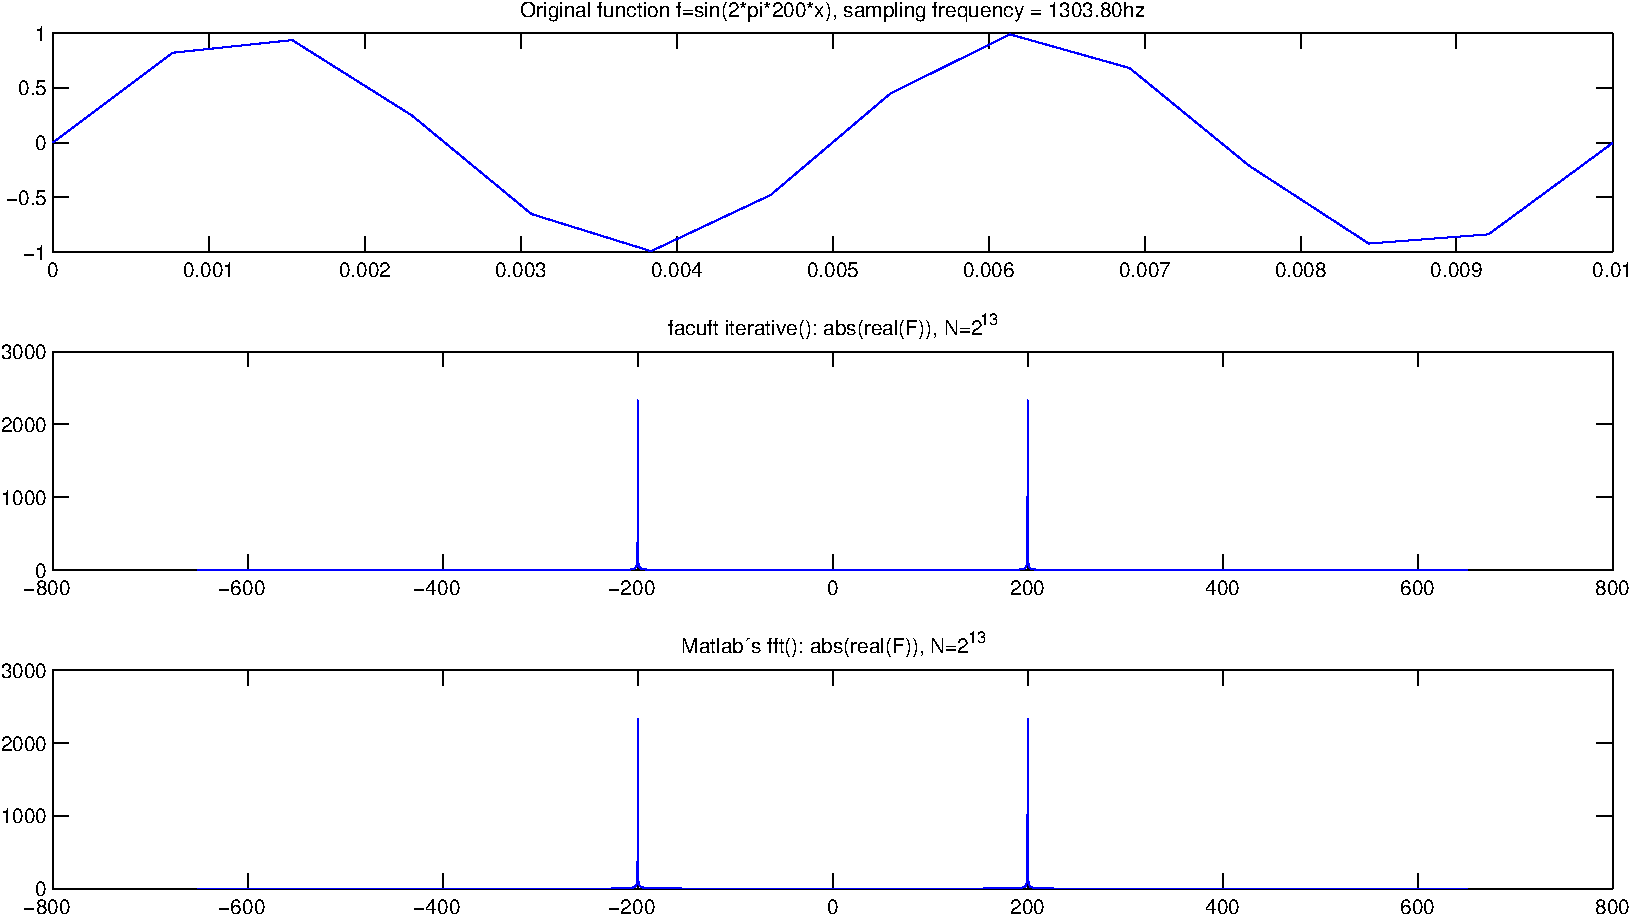
\includegraphics[height=200pt]{img/facuft_iterative}
\end{myframe}

\begin{myframe}{Iterative FFT: Empirical running time}
\centering
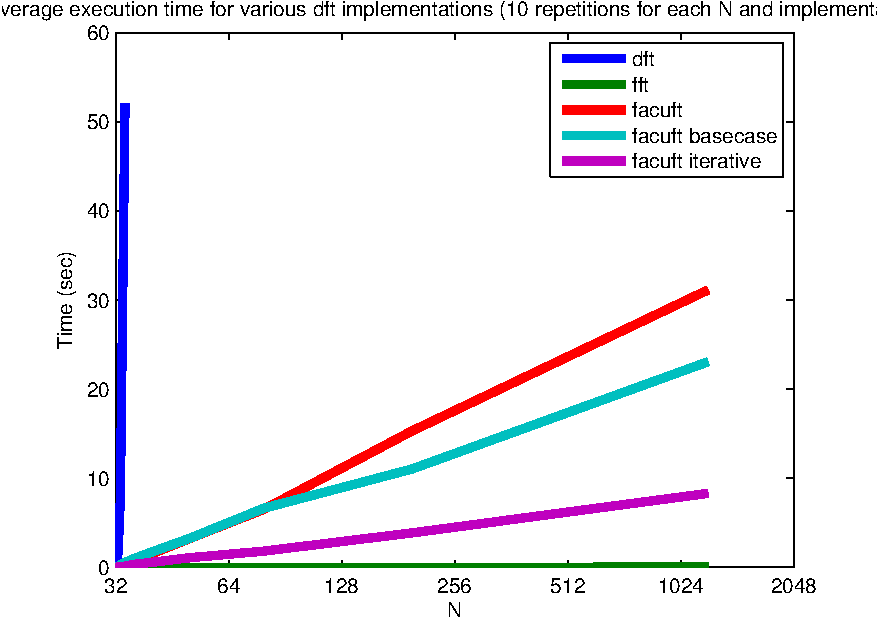
\includegraphics[height=200pt]{img/running_time_iterative}
\end{myframe}